\documentclass[11pt,a4paper]{article}

\usepackage[T1]{fontenc}
\usepackage{lmodern}
\usepackage{amsmath,amssymb,amsthm}
\usepackage{hyperref}
\usepackage{geometry}
\usepackage{booktabs}
\usepackage{microtype}
\usepackage{mathtools}
\usepackage{graphicx}
\usepackage{doi}

\input{glyphtounicode}
\pdfgentounicode=1

\geometry{margin=2.5cm}

\hypersetup{
  pdftitle={Bounded Relational Flux and Ramanujan Expansion Do Not Yet Yield a Cascade-Exponent Bound},
  pdfauthor={Jérôme Beau},
  pdfsubject={Cosmochrony admissibility sub-programme, O4},
  pdfkeywords={relational substrate; Born-Infeld saturation; Ramanujan graphs;
    Kesten-McKay measure; valence growth; cascade exponent; spectral admissibility;
    Cheeger inequality},
  hidelinks
}

\newtheorem{theorem}{Theorem}[section]
\newtheorem{proposition}[theorem]{Proposition}
\newtheorem{lemma}[theorem]{Lemma}
\newtheorem{corollary}[theorem]{Corollary}
\theoremstyle{definition}
\newtheorem{hypothesis}[theorem]{Hypothesis}
\newtheorem{openproblem}[theorem]{Open Problem}
\theoremstyle{remark}
\newtheorem{remark}[theorem]{Remark}

\title{Bounded Relational Flux and Ramanujan Expansion Do Not Yet Yield a Cascade-Exponent Bound}
\author{J\'er\^ome Beau\\
\small Independent Researcher; jerome.beau@cosmochrony.org}
\date{August 2026\\[2pt]\small Version 2.0}

\begin{document}

  \maketitle

  \begin{abstract}
    This note examines whether a structural upper bound on the cascade exponent $\beta$ --
    governing the power-law growth $p(n) \sim n^\beta$ of the effective relational valence
    along the Cosmochrony relaxation cascade -- follows from the Born--Infeld flux constraint
    together with the Cheeger isoperimetric inequality for Ramanujan--LPS graphs.
    It does not follow from the stated argument.
    The front-size argument for this route conflates an edge boundary with a vertex boundary,
    applies a Cheeger inequality in the direction it does not support, and drops a diverging
    factor growing like the square root of $p(n)$ in its concluding asymptotic step; none of
    these defects depends on the others.
    Repairing the underlying closure hypothesis into a well-typed exploration process
    additionally requires several structural choices absent from the Born--Infeld axiom
    itself: a persistent cross-rank exploration model on the LPS/Ramanujan substrate, an
    edgewise flux-allocation law, a dimensionless activation threshold, and a mechanism
    converting available boundary flux into realised, non-congested vertex activations.
    Neither candidate host (a weighted multigraph or a simple graph on successive LPS
    generating sets) currently supports a valid cross-rank spectral estimate: at fixed
    modulus the shells are simple only in a finite window, and at varying modulus successive
    shells act on different groups.
    Interpretively, a conditional analysis identifies a further qualitative tension, stacked
    on this unconstructed host: if such a host existed with a single LPS graph's
    isoperimetric profile, and if a fixed positive fraction of the available activation
    budget were realised with target congestion uniformly bounded, strong expansion would
    favour fast, near-geometric exploration of the underlying group, the qualitative opposite
    of the slow polynomial growth a structural exponent bound requires.
    None of these conditions is derived here.
    No claim is made that a structural upper bound on $\beta$ is impossible; only that the
    argument advanced for it does not hold, and that its most natural repair faces an
    identified conditional structural tension rather than a routine technical gap.
    The residual scientific question -- whether, and by what mechanism, bounded relational
    flux constrains the cascade exponent at all -- is restated as a precisely specified open
    problem.
  \end{abstract}

  \noindent\textbf{Keywords:} relational substrate; Born--Infeld saturation; Ramanujan graphs;
  Kesten--McKay measure; valence growth; cascade exponent; mass hierarchy; spectral admissibility;
  Cheeger inequality

  \clearpage
  \tableofcontents

  \clearpage
  \section{Introduction}
    \label{sec:introduction}

    The inter-generational mass hierarchy of charged leptons spans nearly four orders of
    magnitude, with $m_e / m_\tau \approx 3 \times 10^{-4}$.
    Within the Cosmochrony admissibility sub-programme, the \emph{ordering} and
    \emph{functional form} of this hierarchy have been analysed as arising from the
    contraction of the Kesten--McKay spectral support along a variable-valence relaxation
    cascade~\cite{Beau2026a6, Beau2026a7}; the hierarchy's actual numerical magnitude depends
    on the exponent $\beta$ below, which is not derived by that mechanism.
    The mechanism requires that the effective relational valence $p(n)$ of the Ramanujan--LPS
    relaxation graph grows with the cascade rank $n$, and produces the mass amplification
    formula
    \begin{equation}
      \label{eq:intro-mass-ratio}
      \frac{M_i}{M_j}
      \approx
      \left(\frac{|\lambda_i - 1|}{|\lambda_j - 1|}\right)^{2/\beta},
    \end{equation}
    where $\lambda_i$ are fixed ADE eigenvalue levels and $\beta$ is the exponent governing
    $p(n) \sim n^\beta$~\cite{Beau2026a7}.
    Matching~\eqref{eq:intro-mass-ratio} to the observed lepton hierarchy selects
    $\beta^* \in (0.09, 0.13)$, but leaves the value of $\beta$ as a phenomenological input
    rather than a quantity derived from first principles.
    The derivation of $\beta$ from the internal dynamics of the Cosmochrony substrate was
    identified explicitly as the central open problem of the O-series~\cite{Beau2026a7}.

    The present paper examines this problem from a structural perspective.
    It asks whether the Born--Infeld saturation constraint
    \begin{equation}
      \label{eq:intro-bi}
      |\partial_t \chi_v| \leq c_\chi,
    \end{equation}
    which is the capacity axiom [A-cap] of~\cite{Beau2026c}, combined with the Cheeger
    isoperimetric inequality for Ramanujan--LPS graphs, forces a non-trivial restriction on
    the admissible growth of $p(n)$.
    It does not, by the specific argument examined here.

    A candidate two-step argument for such a restriction can be stated: first, translate the
    local flux bound~\eqref{eq:intro-bi} into a global constraint on front expansion via the
    Cheeger inequality; second, under a closure hypothesis relating the effective valence to
    the cumulative exploration of $\Omega_\chi$ (Hypothesis~\ref{hyp:proportionality}),
    integrate the resulting differential inequality to obtain a power-law upper bound on
    $\beta$.
    Section~\ref{sec:subdiffusion} shows that this argument, as it can currently be made
    precise, contains three independent defects (Section~\ref{ssec:defects}), that the closure
    hypothesis it depends on is not yet a well-typed statement on the LPS/Ramanujan substrate
    (Section~\ref{ssec:setup}), and that a repair sufficient to fix both requires several
    further structural choices not supplied by the Born--Infeld axiom or the LPS construction
    (Section~\ref{ssec:repair}).
    No structural upper bound on $\beta$ is established by this route.

    This finding is structurally non-trivial in its own right.
    Prior to this examination, the two-step argument above was treated in the admissibility
    sub-programme as delivering a structural bound $\beta \leq 2$ (in the raw exponent
    convention of $p(n) \sim n^\beta$; see Remark~\ref{rem:beta-convention}), independent of
    phenomenological calibration.
    That the argument does not establish this removes a claimed structural result from the
    programme's inventory, not merely a technical refinement of one; Section~\ref{ssec:tension}
    additionally identifies a conditional qualitative reason to expect the natural repair
    direction to point away from, rather than toward, the intended slow-growth conclusion.

    The residual scientific question is not closed by this finding.
    Whether, and by what mechanism, bounded relational flux constrains the cascade exponent at
    all is restated precisely as Open Problem~\ref{op:beta-window} in
    Section~\ref{sec:residual}.

    \paragraph{Organisation.}
      Section~\ref{sec:background} recalls the necessary background on the Cosmochrony
      relaxation cascade, Ramanujan--LPS graphs, and the Born--Infeld flux constraint.
      Section~\ref{sec:subdiffusion} states the closure hypothesis and its well-typedness gap,
      presents the three independent defects of the front-size argument, itemises what a
      repair would additionally require, and gives the interpretive tension bearing on the
      likely direction of any repair.
      Section~\ref{sec:residual} restates the residual open problem and the structural
      directions that could supply a genuine bound.
      Section~\ref{sec:pheno} recalls the phenomenological window of O3 for reference.
      Section~\ref{sec:conclusion} summarises the findings and positions this note within the
      O-series.

  \section{Background and Notation}
  \label{sec:background}

  This section recalls the three structural ingredients on which the main argument of
  Section~\ref{sec:subdiffusion} rests: the Cosmochrony relaxation cascade and its
  associated valence parameter, the Ramanujan--LPS graph family and its spectral properties,
  and the Born--Infeld flux constraint.
  No new results are introduced here; the purpose is to fix notation and to make the paper
  self-contained at the level required for the proof.

  \subsection{The relaxation cascade and effective valence}
    \label{ssec:cascade}

    Within the Cosmochrony framework~\cite{Cosmochrony}, effective physical observables
    arise through a non-injective projection
    \begin{equation}
      \Pi : \Omega_\chi \to \mathcal{O},
    \end{equation}
    where $\Omega_\chi$ is the relational configuration space of the pre-geometric substrate
    $\chi$ and $\mathcal{O}$ is the space of effective observables.
    The non-injectivity of $\Pi$ is not a defect but a structural feature: it motivates
    bounded projective capacity, emergent gauge structure, and the finite descriptive
    resolution of the effective theory~\cite{Beau2026c}.

    The relaxation process on $\Omega_\chi$ is organised into a discrete cascade indexed by
    rank $n \in \mathbb{N}$.
    At each rank $n$, the relational connectivity of the substrate is encoded in a relaxation
    graph $\mathcal{G}(n)$, whose vertices represent admissible relational configurations and
    whose edges represent elementary update steps compatible with the bounded-flux constraint.
    The cascade rank $n$ is not a time coordinate but an organisational depth parameter
    measuring how far the relaxation has propagated into $\Omega_\chi$.

    The degree of $\mathcal{G}(n)$ is denoted $d(n) = p(n) + 1$, where $p(n)$ is the
    effective valence parameter at rank $n$.
    In the fixed-valence regime $p(n) = p$ for all $n$, the Kesten--McKay spectral support
    of $\mathcal{G}(n)$ is constant, and the projective resolution threshold $\Lambda_{\mathrm proj}(n)$
    saturates asymptotically~\cite{Beau2026a5}.
    This saturation prevents the generation of a non-trivial inter-level hierarchy from fixed
    spectral data alone.
    The variable-valence regime $p(n) \to \infty$ was introduced in~\cite{Beau2026a6} as the
    minimal dynamical extension that removes this obstruction: as $p(n)$ grows, the
    Kesten--McKay support contracts toward its midpoint $\lambda = 1$, causing the fixed ADE
    eigenvalue levels to exit the support at distinct, rank-dependent thresholds.

    Throughout this paper, the growth law is assumed to be of power-law form,
    \begin{equation}
      \label{eq:power-law}
      p(n) \sim n^\beta
      \qquad \text{as } n \to \infty,
    \end{equation}
    with $\beta > 0$ to be constrained.
    The case $\beta = 0$ (bounded valence) recovers the fixed-valence saturation regime
    of~\cite{Beau2026a5} and is excluded from the present analysis.

    \begin{figure}[h]
      \centering
      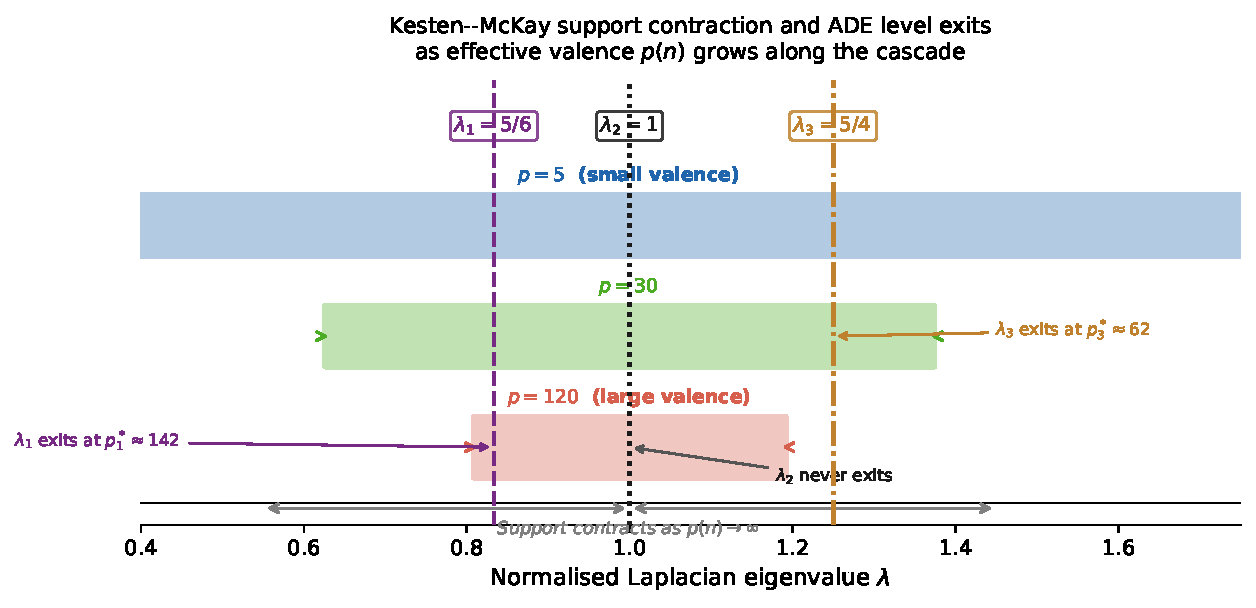
\includegraphics[width=0.92\textwidth]{../code/fig1_km_contraction}
      \caption{Kesten--McKay spectral support (coloured bands) at three representative
      valence values $p = 5, 30, 120$, superimposed on the three fixed ADE eigenvalue
      levels $\lambda_1 = 5/6$, $\lambda_2 = 1$, $\lambda_3 = 5/4$.
      As $p(n)$ grows, the support $[1 - 2/\sqrt{p},\, 1 + 2/\sqrt{p}]$ contracts toward
      its midpoint $\lambda = 1$.
      The level $\lambda_3 = 5/4$ exits the support first at $p^*_3 \approx 62$;
        $\lambda_1 = 5/6$ exits second at $p^*_1 \approx 142$;
        $\lambda_2 = 1$ never exits.
        This ordered exit sequence is the spectral mechanism~\cite{Beau2026a6} producing an
        ordered separation of the three levels, conventionally read as an effective mass
        ordering $M_3 > M_1 > M_2$ conditional on the level-to-generation identification --
        itself not established from first principles~\cite{Beau2026a6} -- and independent of
        the front-size argument examined in this note.}
      \label{fig:km-contraction}
    \end{figure}

  \subsection{Ramanujan--LPS graphs}
    \label{ssec:lps}

    The relaxation graphs $\mathcal{G}(n)$ are taken to be Cayley graphs of
    $\mathrm{PSL}(2, \mathbb{F}_q)$ constructed by the Lubotzky--Phillips--Sarnak (LPS)
    method~\cite{LPS}, with degree $d = p + 1$ determined by a prime $p \equiv 1 \pmod{4}$.
    These graphs are $(p+1)$-regular and satisfy the Ramanujan property: every non-trivial
    adjacency eigenvalue $\mu$ satisfies
    \begin{equation}
      \label{eq:ramanujan}
      |\mu| \leq 2\sqrt{p}.
    \end{equation}
    Equivalently, the normalised Laplacian eigenvalues $\lambda = 1 - \mu/(p+1)$ of
    non-trivial sectors satisfy the two-sided bound
    \begin{equation}
      \label{eq:ramanujan-laplacian}
      \left(\sqrt{p} - 1\right)^2 \leq \lambda \cdot (p+1) \leq \left(\sqrt{p} + 1\right)^2,
    \end{equation}
    an algebraic restatement of~\eqref{eq:ramanujan} under $\lambda=1-\mu/(p+1)$: both sides
    of this two-sided bound are the Ramanujan property itself, established for the LPS
    family via Deligne's theorem on the Ramanujan--Petersson conjecture, following~\cite{LPS},
    not the content of the Alon--Boppana theorem.
    Alon--Boppana~\cite{AlonBoppana} is a separate, related fact: for \emph{any} infinite
    family of $(p+1)$-regular graphs of growing size, the spectral gap cannot do
    asymptotically better than $2\sqrt p$, so the Ramanujan property here is asymptotically
    optimal, not merely one admissible bound among many; it is not itself a source of either
    side of~\eqref{eq:ramanujan-laplacian}.

    The spectral gap of $\mathcal{G}(n)$ satisfies
    $\lambda_2 \geq (\sqrt{p(n)} - 1)^2 / (p(n) + 1)$.
    Here $h(\mathcal{G}(n))$ denotes the \emph{unnormalised} edge-isoperimetric (Cheeger)
    constant, defined so that for any subset $S$ of vertices with $|S| \leq |\mathcal{G}(n)|/2$,
    the edge boundary satisfies $|\partial S| \geq h(\mathcal{G}(n)) \cdot |S|$.
    For a $d$-regular graph, the discrete Cheeger inequality relates this unnormalised
    constant to the normalised Laplacian spectral gap $\lambda_2$ via a factor of the
    degree~\cite{Cheeger, HLW}:
    \begin{equation}
      \label{eq:cheeger-background}
      h(\mathcal{G}(n))
      \;\geq\;
      \frac{d(n)\,\lambda_2(\mathcal{G}(n))}{2}
      \;\gtrsim\;
      \frac{(p(n)+1)\,(\sqrt{p(n)} - 1)^2}{2(p(n) + 1)}
      \;=\;
      \frac{(\sqrt{p(n)}-1)^2}{2}
      \;\sim\;
      \frac{p(n)}{2},
    \end{equation}
    i.e.\ $h(\mathcal{G}(n))$ grows linearly in $p(n)$, not toward a constant, as
    $p(n) \to \infty$.
    (The front-size argument audited in Section~\ref{ssec:defects} uses instead the
    unnormalised-looking but degree-free estimate $h(\mathcal{G}(n)) \gtrsim
    1 - 1/\sqrt{p(n)}$, which omits this degree factor; Defect 3 audits that argument's own
    algebra using its own stated quantity, without endorsing it as the correct value.)

    The LPS construction is used here because it provides an explicit, analytically tractable
    Ramanujan family whose spectral properties are uniform in $p$ and whose generating
    structure is compatible with the admissibility framework of~\cite{Beau2026a1}.
    Section~\ref{sec:subdiffusion} examines an argument for a growth bound on this specific
    family; no such bound is established there, and consequently none is claimed to extend to
    other Ramanujan or expanding-degree families either.

    The LPS graphs used throughout require, beyond $p,q \equiv 1 \pmod 4$ prime and $p \neq q$,
    that $p$ be a quadratic residue modulo $q$ (equivalently, in the Legendre-symbol notation,
    $\left(\tfrac{p}{q}\right) = 1$), which selects the $\mathrm{PSL}(2,\mathbb{F}_q)$
    realisation used here; the non-residue case gives the $(p+1)$-regular
    $\mathrm{PGL}(2,\mathbb{F}_q)$ construction instead, not used in this note.

    A further condition is needed for the graph to genuinely have $p+1$ \emph{distinct}
    generators (equivalently, for the reduction $\Omega_p \to \mathrm{PSL}(2,\mathbb F_q)$ of
    the $p+1$ integer quaternions of norm $p$ to be injective, so that the Cayley graph is
    simple with no repeated or coincident generators).
    The full argument needs the reduction map made precise, not only the final magnitude
    estimate.

    By Jacobi's four-square theorem, under the standard LPS normalisation ($a>0$ odd; $b,c,d$
    even), the equation $a^2+b^2+c^2+d^2=p$ has exactly $p+1$ integer solutions; $\Omega_p$ is
    this set.
    In particular no $\alpha \in \Omega_p$ has $-\alpha \in \Omega_p$ as well, since $a>0$ for
    every element.
    Fix, once and for all, a square root $\bar\imath$ of $-1$ modulo $q$ (exists since
    $q\equiv1\pmod4$) and a single square root $\sqrt p$ of $p$ modulo $q$ (exists by the
    quadratic-residue condition above), used uniformly for every $\alpha\in\Omega_p$ -- not
    chosen independently per element.
    Each $\alpha=(a,b,c,d)$ maps to
    \[
    M(\alpha) \;=\; \begin{pmatrix} a+b\bar\imath & c+d\bar\imath \\ -c+d\bar\imath &
    a-b\bar\imath \end{pmatrix} \pmod q,
    \]
    of determinant $a^2+b^2+c^2+d^2=p \equiv (\sqrt p)^2 \pmod q$; dividing by the fixed
    $\sqrt p$ gives an element of $\mathrm{SL}(2,\mathbb F_q)$, and the further quotient by the
    centre $\{\pm I\}$ gives the class of $\alpha$ in $\mathrm{PSL}(2,\mathbb F_q)$.

    The map $\alpha \mapsto M(\alpha) \bmod q$ is injective component-wise: from the diagonal
    entries, $a \equiv (M_{11}+M_{22})/2$ and $b \equiv (M_{11}-M_{22})/(2\bar\imath) \pmod q$
    (both $2$ and $\bar\imath$ invertible modulo the odd prime $q$), and $c,d$ recover
    symmetrically from the off-diagonal entries; so $M(\alpha)\equiv M(\alpha')\pmod q$ if and
    only if $\alpha\equiv\alpha'\pmod q$ component-wise.
    Two elements $\alpha,\alpha'\in\Omega_p$ give the \emph{same} class in
    $\mathrm{PSL}(2,\mathbb F_q)$ if and only if $M(\alpha)/\sqrt p \equiv \pm
    M(\alpha')/\sqrt p \pmod q$ -- the projective scalar in the $\mathrm{SL}\to\mathrm{PSL}$
    quotient reduces to $\pm1$ -- equivalently (the fixed, common $\sqrt p$ being invertible
    mod $q$, and by the component-wise injectivity just shown) $\alpha \equiv \pm\alpha'
    \pmod q$ as integer quaternions.

    Two distinct $\alpha,\alpha' \in \Omega_p$ have components bounded by $\sqrt p$ in
    absolute value, so every component of $\alpha \mp \alpha'$ lies in the open interval
    $(-2\sqrt p,\, 2\sqrt p)$; if $q > 2\sqrt p$, no nonzero integer in that range is
    $\equiv 0 \pmod q$, so each congruence $\alpha\equiv\alpha'\pmod q$ or
    $\alpha\equiv-\alpha'\pmod q$ forces the corresponding \emph{integer} equality,
    $\alpha=\alpha'$ or $\alpha=-\alpha'$.
    The second case is impossible for $\alpha\neq0$: $\alpha=-\alpha'$ would need $a=-a'$ with
    $a,a'>0$, excluded by the sign normalisation recalled above.
    Hence $q > 2\sqrt p$ forces $\alpha=\alpha'$ whenever $\alpha,\alpha'\in\Omega_p$ have the
    same $\mathrm{PSL}(2,\mathbb F_q)$ image: it is a sufficient injectivity condition,
    guaranteeing $p+1$ pairwise distinct generators after reduction.

    Since the variable-valence LPS sequence's own defining requirement $p(n) \to \infty$
    forces this condition to be checked at every rank, a variable-valence sequence compatible with
    simplicity throughout requires $q(n) \gtrsim \sqrt{p(n)}$ -- a growth rate for $q(n)$ that
    is not stated in the companion paper introducing the sequence~\cite{Beau2026a6}, and is
    strictly stronger than the weaker cardinality bound $q(n) \gtrsim p(n)^{1/3}$ needed merely
    for $\mathrm{PSL}(2,\mathbb F_{q(n)})$ to be large enough to contain $p(n)+1$ elements at
    all.
    This condition is stated here for completeness; it does not by itself resolve any of the
    findings of Section~\ref{sec:subdiffusion}, which concern the front-size argument and the
    exploration host's own construction (Remark~\ref{rem:hyp-status}) rather than the
    generator-distinctness question addressed here.

  \subsection{The Born--Infeld flux constraint}
    \label{ssec:bi}

    The bounded-flux constraint is the capacity axiom [A-cap] of~\cite{Beau2026c}:
    an explicit structural hypothesis, motivated by non-injective projection with finite
    local distinguishability.
    In its discrete form, it reads
    \begin{equation}
      \label{eq:bi-background}
      |\partial_t \chi_v| \leq c_\chi
      \qquad \text{for every node } v \in \mathcal{G}(n),
    \end{equation}
    where $\chi_v$ is the value of the relational field at node $v$ and $c_\chi$ is the
    universal saturation scale.

    Equation~\eqref{eq:bi-background} is a local bound: it restricts the rate of change of
    $\chi$ at each node independently, without direct reference to the global structure of
    $\mathcal{G}(n)$.
    Its global consequences are non-trivial and are the subject of the present paper.

    The physical content of~\eqref{eq:bi-background} is that the relational substrate cannot
    update arbitrarily fast: there is a maximal admissible rate of change of $\chi$ at any
    single node, not a per-edge or per-channel bound (see Defect 2, Section~\ref{ssec:defects},
    for where the front-size argument conflates the two).
    In the continuum limit, a Born--Infeld-type effective action is the saturation
    candidate compatible with this bound~\cite{Beau2026c}, much as the finiteness of the
    speed of light distinguishes special relativity from Galilean mechanics.
    In the discrete cascade setting, it is intended to translate into a bound on the rate at
    which the relaxation can explore new regions of $\Omega_\chi$; Section~\ref{ssec:defects}
    examines an argument for such a bound and shows it does not hold as stated.

    The scale $c_\chi$ appears in~\eqref{eq:bi-background} as a universal constant.
    Section~\ref{sec:subdiffusion} examines whether any bound on $\beta$ follows from
    $c_\chi$'s finiteness together with the Ramanujan graphs' isoperimetric property; no such
    bound is established there.

  \section{The Front-Size Argument and Why It Does Not Establish a Growth Bound}
  \label{sec:subdiffusion}

  \subsection{Setup and closure hypothesis}
    \label{ssec:setup}

    At cascade rank $n$, the relaxation graph $\mathcal{G}(n)$ is a Ramanujan--LPS Cayley
    graph of degree $d(n) = p(n) + 1$, where $p(n)$ is the effective valence parameter at
    that rank.
    The bounded-flux constraint inherited from the Born--Infeld substrate reads
    \begin{equation}
      \label{eq:bi-constraint}
      |\partial_t \chi_v| \leq c_\chi
      \qquad
      \text{for every node } v \in \mathcal{G}(n).
    \end{equation}

    Equation~\eqref{eq:bi-constraint} bounds the relational flux locally but does not by
    itself specify how the effective valence $p(n)$ grows along the cascade.
    To connect bounded flux with valence growth, we introduce the following closure hypothesis.

    \begin{hypothesis}[Valence--exploration proportionality]
      \label{hyp:proportionality}
      For the changing-valence LPS relaxation family considered in this paper,
      the effective relational valence $p(n)$ is proportional to the cumulative number
      $N(n)$ of distinct relational configurations reached by the relaxation process up to
      cascade rank $n$:
      \begin{equation}
        \label{eq:proportionality}
        p(n) \propto N(n).
      \end{equation}
    \end{hypothesis}

    \begin{remark}
      \label{rem:hyp-status}
      Hypothesis~\ref{hyp:proportionality} is a closure assumption, not a microscopic
      dynamical law.
      Within the Cosmochrony framework, each newly reached node of $\Omega_\chi$ corresponds
      to a distinct admissible relational configuration, and therefore contributes one new
      effective channel in the relaxation graph.
      The hypothesis states only that these contributions accumulate proportionally; it does
      not fix the rate of exploration, which remains entirely encoded in the bounded-flux
      constraint~\eqref{eq:bi-constraint}.
      In particular, $\beta$ is not an input to Hypothesis~\ref{hyp:proportionality}: no
      assumption on the growth rate of $p(n)$ is made at this stage.
      The hypothesis is expander-scoped.  It does not transfer to the fixed-degree
      Heisenberg BFS cascade, where the two native corpus realisations contradict the
      required proportionality; see the Span-Growth Note
      \href{https://doi.org/10.5281/zenodo.21480521}{doi:10.5281/zenodo.21480521}.

      $N(n)$ is characterised above only by the informal description ``the cumulative number
      of distinct relational configurations reached... up to cascade rank $n$.''
      No combinatorial definition or recurrence for $N(n)$ is given independent of the
      front-size argument of Section~\ref{ssec:defects} that uses it.
      In particular, the host object on which $N(n)$ is meant to grow -- a single, persistent
      structure accumulating explored configurations as the LPS parameter $p(n)$ increases --
      is not supplied by the variable-valence LPS sequence of the companion paper introducing
      it~\cite{Beau2026a6} (a sequence of graphs on generally distinct, non-nested vertex
      sets), nor by the standard LPS generator construction at fixed vertex set (whose
      integer-quaternion source shells at distinct fixed norms do not nest by construction;
      whether their reduced generator images in $\mathrm{PSL}(2,\mathbb F_q)$ do is a
      separate, open number-theoretic question).
      Hypothesis~\ref{hyp:proportionality} is therefore not yet a well-typed mathematical
      statement on this substrate: it names a relation between two quantities before one of
      them has an agreed construction.
    \end{remark}

    \begin{remark}[Notation: $\beta$ denotes the raw exponent throughout]
      \label{rem:beta-convention}
      Throughout this note, $\beta$ denotes the same exponent used in
      O3~\cite{Beau2026a7} and defined in~\eqref{eq:power-law}: the raw exponent of
      $p(n) \sim n^\beta$, matching~\eqref{eq:intro-mass-ratio}'s exponent $2/\beta$.
      No rescaled exponent is introduced.
      In this convention, the candidate quadratic bound $p(n) \lesssim C n^2$ examined in
      Section~\ref{ssec:defects} would correspond to $\beta \leq 2$, not $\beta \leq 1$: a
      rescaling $\tilde\beta := \beta/2$ would map the candidate bound to $\tilde\beta \leq 1$,
      but would equally rescale O3's window to $\tilde\beta^* \in (0.045, 0.065)$, not leave it
      at $(0.09, 0.13)$.
      Stating both the candidate bound and O3's window in the same, unrescaled $\beta$ avoids
      this inconsistency.
    \end{remark}

  \subsection{Three independent defects of the front-size argument}
    \label{ssec:defects}

    A candidate argument for a growth bound proceeds as follows: under the bounded-flux
    constraint~\eqref{eq:bi-constraint} on a Ramanujan--LPS graph $\mathcal{G}(n)$ of degree
    $p(n)+1$, bound the number of newly reachable nodes at cascade rank $n$ by
    $\Delta N(n) \lesssim c_\chi \sqrt{p(n)}$, then integrate under
    Hypothesis~\ref{hyp:proportionality} to obtain a power-law upper bound on $p(n)$.
    This argument contains three independent defects, each sufficient on its own to
    invalidate it; none depends on the others, and repairing any one alone does not repair
    the argument.

    \begin{enumerate}
      \item[\textbf{Defect 1 (boundary-type mismatch).}]
        Section~\ref{ssec:lps}'s own definition of $\partial S$ (edge boundary, entering the
        quoted Cheeger inequality~\eqref{eq:cheeger-background}) and a set $S_n$ of explored
        configurations' boundary $\partial S_n$ as used in the front-size argument (there
        taken to be the set of \emph{nodes} not yet in $S_n$ adjacent to $S_n$) are different
        objects on a degree-$(p(n)+1)$ graph.
        Converting between an edge-boundary cardinality and a vertex-boundary cardinality
        needs a degree-dependent factor that is not supplied by the argument.

      \item[\textbf{Defect 2 (wrong-direction inequality).}]
        The Cheeger inequality available here,
        $|\partial S| \geq h(\mathcal{G}(n))\,|S|$, is a \emph{lower} bound on boundary size.
        It does not, by itself or via any stated intermediate step, yield an \emph{upper}
        bound on the number of newly reached vertices.
        The local flux bound~\eqref{eq:bi-constraint} constrains total outgoing flux from a
        node, not the number of vertices that flux can activate, without an explicit
        minimum-flux-per-activation threshold -- which the argument does not introduce.
        A further, independent gap sits inside the argument's own intermediate step: the
        node-level bound $|\partial_t \chi_v| \leq c_\chi$ is a rate at the node, not a
        per-edge or per-channel quantity, so ``the total outgoing flux from any node through
        its boundary edges is at most $(p(n)+1)\,c_\chi$'' -- used to obtain Defect 3's
        estimate below -- already presupposes an edgewise allocation of the node bound (each
        of the $p(n)+1$ channels carrying up to $c_\chi$) that is not itself part of
        $[\text{A-cap}]$'s statement (cf.\ item~3 of Section~\ref{ssec:repair}).

      \item[\textbf{Defect 3 (asymptotic error).}]
        Even granting the unsupported upper bound of Defect 2, combining the (unjustified)
        total outgoing flux estimate $(p(n)+1)\,c_\chi$ with the argument's own quoted
        Cheeger estimate $h(\mathcal{G}(n)) \gtrsim 1-1/\sqrt{p(n)}$ -- the degree-free
        estimate flagged in Section~\ref{ssec:lps} as omitting the degree factor of the
        correct discrete Cheeger inequality~\eqref{eq:cheeger-background}, quoted here only
        because it is what the argument itself uses -- yields an estimate of order
        $c_\chi\, p(n)$, not $c_\chi\sqrt{p(n)}$: the ratio between the two,
        $\sqrt{p(n)}/(1-1/\sqrt{p(n)})$, diverges like $\sqrt{p(n)}$ as $p(n)\to\infty$, so
        treating it as an $O(1)$ constant silently drops a diverging factor.
        (Substituting the corrected, degree-inclusive Cheeger estimate of
        Section~\ref{ssec:lps} would change this intermediate number again, but does not
        rescue the argument: Defects 1 and 2 already invalidate it independently of this
        estimate's value.)
    \end{enumerate}

  \subsection{What a repair would additionally require}
    \label{ssec:repair}

    Beyond Hypothesis~\ref{hyp:proportionality}'s own well-typedness gap
    (Remark~\ref{rem:hyp-status}) and the three defects of
    Section~\ref{ssec:defects}, a repaired argument would additionally require the following,
    none of which is supplied by the Born--Infeld axiom or the LPS construction:

    \begin{enumerate}
      \item a persistent cross-rank exploration host on which a valid spectral estimate can
        be run at all: at fixed $q$, generator shells are simple only within the finite
        window $q>2\sqrt{p(n)}$ (Section~\ref{ssec:lps}), and a union of \emph{generating
        sets} is not the same object as a cumulative set of \emph{explored vertices}; at
        variable $q(n)$ -- the regime the variable-valence LPS sequence requires for
        unbounded $p(n)\to\infty$ -- successive shells act on different groups
        $\mathrm{PSL}(2,\mathbb F_{q(k)})$, so no common spectral estimate across ranks is
        even meaningful (Section~\ref{ssec:tension} details both obstructions);
      \item independently of item~1, a resolution of whether such a host, if constructed,
        should be a weighted multigraph (with edge multiplicities requiring their own
        physical interpretation as parallel relational channels) or a simple graph (requiring
        a proved bound on cross-generator overlap, not currently available);
      \item an edgewise flux-allocation law converting the node-level bound
        $|\partial_t\chi_v|\leq c_\chi$ into a per-edge quantity, a choice not fixed by
        [A-cap]'s own statement;
      \item an activation threshold $\epsilon_0 = \kappa c_\chi$, with $\kappa$ dimensionless
        as required within the current admissibility contract so as not to introduce an
        independent dimensional scale, whose numerical value is not fixed by anything in this
        note;
      \item an activation-utilisation law and a target-congestion bound, since availability
        of boundary flux does not by itself force realised, non-overlapping vertex
        activations.
    \end{enumerate}

    This is not a claim that such a repair is impossible: it names what is currently missing,
    so that a future construction can be checked against an explicit list rather than
    assembled piecemeal.

  \subsection{Interpretation: expansion and the direction of the missing argument}
    \label{ssec:tension}

    The defects of Section~\ref{ssec:defects} leave open whether a structural bound on
    $\beta$ exists via some other argument.
    A further consideration bears on which direction any repair is likely to point, even
    though it does not settle the question.

    \paragraph{Why a cross-rank spectral estimate is not available.}
    Section~\ref{ssec:repair} names, as candidate constructions for the missing exploration
    host, a weighted multigraph on the multiset union $M_n := \biguplus_{k\leq n} S_{p(k),q}$
    of successive LPS generating sets, or a simple graph on their set union $T_n :=
    \bigcup_{k\leq n} S_{p(k),q}$.
    Neither currently supports a valid cross-rank spectral estimate.
    At fixed $q$, the individual shells $S_{p(k),q}$ are simple and injective only while
    $q > 2\sqrt{p(k)}$ (Section~\ref{ssec:lps}), so any sum over $k\leq n$ is restricted to a
    finite window in $n$, not an asymptotic statement; moreover $M_n$ or $T_n$ (a set of
    \emph{generators}, controlling the degree of a Cayley graph) is not the same object as a
    cumulative set of \emph{explored vertices} on that graph, and the two must not be
    identified.
    At variable $q(n)$ -- the regime the variable-valence LPS sequence actually requires for
    $p(n)\to\infty$ unboundedly -- the operators $A(S_{p(k),q(k)})$ for different $k$ act on
    $L^2$ of
    \emph{different} groups $\mathrm{PSL}(2,\mathbb F_{q(k)})$, so no operator sum or common
    spectral estimate across $k$ is even meaningful.
    Both routes are closed as stated; no weighted-union or simple-union spectral bound is
    used below.

    \paragraph{What a single LPS graph's isoperimetry gives, if a host existed.}
    What remains valid is the single-graph fact of Section~\ref{ssec:lps}: for the one
    Ramanujan--LPS graph $\mathcal G(n)$ of degree $d(n)=p(n)+1$ at a given rank (not a union
    across ranks), the normalised edge conductance
    \[
    \varphi(\mathcal G(n)) \;:=\; \frac{h(\mathcal G(n))}{d(n)}
    \;\gtrsim\; \frac{(\sqrt{p(n)}-1)^2}{2(p(n)+1)} \;\to\; 1/2
    \]
    is bounded away from $0$ as $p(n)\to\infty$, using~\eqref{eq:cheeger-background} directly
    (no vertex-isoperimetric detour, and no union).
    For any vertex subset $E \subseteq \mathcal G(n)$ with $|E|\leq|\mathcal G(n)|/2$, the edge
    boundary satisfies $|\partial E| \geq h(\mathcal G(n))|E|$, and since each inner-boundary
    vertex contributes at most $d(n)$ edges to $\partial E$,
    \begin{equation}
      \label{eq:tension-inner}
      |\partial^-_V E| \;\geq\; \frac{|\partial E|}{d(n)} \;\geq\; \varphi(\mathcal G(n))\,|E|,
    \end{equation}
    with $\varphi(\mathcal G(n))$ bounded below by a positive constant -- this is the
    corrected route from a normalised edge quantity to the inner vertex boundary, not the
    vertex-isoperimetric constant used in an earlier draft of this argument, which does not
    itself stay bounded away from $0$ relative to the degree.

    \paragraph{The conditional bound, on an explicitly unconstructed host.}
    \eqref{eq:tension-inner} says something about a \emph{single} graph, not about a
    cumulative exploration process; using it for the latter requires, in addition to items
    1--2 of Section~\ref{ssec:repair} (a persistent host and its simple-vs-multigraph
    resolution, neither supplied), items 3--5 (an edgewise flux-allocation law; the
    activation threshold $\epsilon_0=\kappa c_\chi$ with $\kappa$ dimensionless and
    $0<\kappa\leq1$, so $b(n):=\min(p(n)+1,\lfloor1/\kappa\rfloor)\geq1$; and an
    activation-utilisation and target-congestion mechanism).
    \emph{If} a persistent host $E_n$ existed with the isoperimetric profile of a single LPS
    graph at each rank, \emph{and} a fixed fraction $\eta\in(0,1]$ of each inner-boundary
    vertex's budget $b(n)$ were realised, \emph{and} each exterior target vertex absorbed at
    most $C_n$ realised activations, then, while $|E_n|\leq|\mathcal G(n)|/2$,
    \begin{equation}
      \label{eq:tension-bound}
      \Delta|E_n| \;\geq\; \frac{\eta\,b(n)}{C_n}\,\varphi(\mathcal G(n))\,|E_n|,
    \end{equation}
    and if $\eta$, $b(n)$, and $1/C_n$ are further bounded below by positive constants, this
    is a geometric recursion reaching the volume threshold on a depth scale logarithmic in
    $|\mathcal G(n)|$ -- not the polynomial growth $p(n)\sim n^\beta$ a structural exponent
    bound presupposes -- saying nothing about what happens beyond that threshold.

    This is a \textbf{conditional result stacked on an unconstructed premise}, not merely an
    unproved claim about an existing object: even granting $\eta$ and $C_n$ bounded as
    stated, \eqref{eq:tension-bound} presupposes the host $E_n$ itself, which
    Section~\ref{ssec:repair} and the paragraph above show is not currently supplied by either
    candidate construction.
    The qualitative point survives this scoping: \emph{if} a well-defined exploration process
    on this substrate inherits a single LPS graph's isoperimetric profile at all, geometric
    rather than polynomial growth is the generic expectation, not an assumption smuggled in to
    reach a desired conclusion -- but no construction in this note or its sources currently
    supplies that host, so the qualitative point is exactly that: qualitative, not a
    derivation with a stated remaining gap in $\eta$ and $C_n$ alone.

  \section{The Residual Problem and its Geometric Content}
  \label{sec:residual}

  \subsection{Scope of the open problem}
    \label{ssec:scope}

    Section~\ref{sec:subdiffusion} examined whether the bounded-flux
    constraint~\eqref{eq:bi-constraint} restricts valence growth to $p(n) \lesssim C n^2$,
    i.e.\ to at most quadratic cumulative exploration, written $\beta \leq 2$ in the raw
    exponent convention of Remark~\ref{rem:beta-convention}.
    No such bound is established there: Section~\ref{ssec:defects} identifies three
    independent defects in the argument advanced for it, and Section~\ref{ssec:repair}
    identifies what a repair would additionally require.
    Consequently, even the qualitative claim that Born--Infeld saturation slows the
    exploration of the relational configuration space is open, not merely the sharper
    quantitative confinement discussed below.

    The companion paper O3~\cite{Beau2026a7} identifies, from the charged-lepton mass ratios,
    the narrow phenomenological window $\beta^* \in (0.09, 0.13)$, in the same raw-exponent
    convention.
    \emph{If} a structural upper bound $\beta \leq 2$ were established by a repaired argument,
    it would be compatible with this window without explaining it: the gap between the two
    would be a factor of roughly $15$--$22$ in the exponent ($2/0.13 \approx 15.4$ to
    $2/0.09 \approx 22.2$), itself requiring further structure to close.
    This note does not establish the premise of that conditional.

  \subsection{Three sources of additional structure}
    \label{ssec:three-sources}

    We identify three independent directions that could supply the missing confinement.

    \paragraph{Effective dimension of $\Omega_\chi$.}
      The closure Hypothesis~\ref{hyp:proportionality} treats the exploration of $\Omega_\chi$
      as essentially one-dimensional along the cascade.
      If the relational configuration space has an effective intrinsic dimension $D > 1$ and,
      in addition, cascade rank advances a ball radius at a fixed rate ($r \sim n$, a
      rank-to-radius law not established anywhere in this note or its sources), a standard
      volume-growth relation $N \sim r^D$ would give $N(n) \sim n^D$; neither the dimension
      $D$ nor the rank-to-radius law is supplied, so this scaling is not asserted here, only
      identified as a possible source of a tighter front bound if both were established.
      Determining $D$ from the spectral structure of $\mathcal{G}(n)$, and separately deriving
      a rank-to-radius law, are open problems; the former is amenable to the spectral
      reconstruction techniques of~\cite{Beau2026a}, the latter is not addressed by that
      reference.

    \paragraph{A genuinely Born--Infeld/DBI dynamical model.}
      The front-size argument examined in Section~\ref{ssec:defects} does not use any
      linearised or saturated regime of a Dirac--Born--Infeld action: it uses only the flat
      capacity bound $[\text{A-cap}]$, $|\partial_t \chi_v| \leq c_\chi$, directly.
      A genuinely different direction would replace this hard bound by an explicit nonlinear
      DBI equation of motion for $\chi_v$, of which $[\text{A-cap}]$ is at best an asymptotic
      or saturation feature rather than the starting hypothesis, extending the one-mode
      reduction of~\cite{Beau2026a1} to the variable-valence setting.
      Whether such a model constrains front growth more tightly than
      Section~\ref{ssec:defects}'s (invalid) argument is open; a dimensionally consistent
      bound of this kind would need to introduce whatever second scale the nonlinear DBI
      action itself supplies, since $c_\chi^\alpha \sqrt{p(n)}$ for $\alpha \neq 1$ is not
      well-typed on $c_\chi$ alone without one.

    \paragraph{Spectral mixing time and cascade coherence.}
      Requiring that the relaxation at rank $n$ reaches spectral equilibrium before rank $n+1$
      imposes a constraint on the mixing time of $\mathcal{G}(n)$.
      For Ramanujan graphs, the mixing time is controlled by the spectral gap and the graph
      diameter.
      Translating this coherence requirement into a bound on $p(n)$ requires a precise model of
      the time parameterisation along the cascade, which is currently absent.
      This direction is now a candidate \emph{explanation} for the difficulty identified in
      Section~\ref{ssec:tension}, not merely a possible refinement: if bounded flux and strong
      expansion generically favour fast, mixing-time-scale exploration, a coherence constraint
      of this kind is the most plausible remaining mechanism by which slow growth could still
      be enforced, and is accordingly the natural target for the next step of the programme.

  \subsection{Summary of the residual open problem}
  \label{ssec:open-problem}

  The residual problem may be stated precisely as follows.

  \begin{openproblem}[Structural derivation of the phenomenological window]
    \label{op:beta-window}
    Derive, from the geometry of $\Omega_\chi$ and the Born--Infeld saturation dynamics of
    $\chi$, an upper bound of the form
    \begin{equation}
      \beta \leq \beta_{\mathrm{struct}} \ll 1,
    \end{equation}
    where $\beta_{\mathrm{struct}}$ is determined solely by intrinsic, dimensionless
    parameters of the Cosmochrony substrate --- such as the effective dimension $D$ of
    $\Omega_\chi$ and dimensionless spectral invariants of $\mathcal{G}(n)$ --- and is
    numerically compatible with the phenomenological window $\beta^* \in (0.09, 0.13)$.
    Since $\beta_{\mathrm{struct}}$ is itself dimensionless, the dimensionful saturation scale
    $c_\chi$ cannot enter alone; it could only contribute through a dimensionless ratio with
    some other scale, none of which this note supplies (cf.\ the Level-2 unit-conversion gap
    discussed for $c_\chi$ elsewhere in the audited corpus).
    Here $\beta$ is the raw exponent of Remark~\ref{rem:beta-convention}, matching O3's own
    convention.
  \end{openproblem}

  Open Problem~\ref{op:beta-window} is stated at the level of the sharp phenomenological
  target for concreteness, but Sections~\ref{ssec:defects}--\ref{ssec:tension} establish that
  the weaker goal -- any rigorous structural upper bound on $\beta$ at all, whether or not it
  matches $\beta^*$ -- is presently open as well, not merely insufficiently tight.
  The three directions of Section~\ref{ssec:three-sources} each represent a distinct path
  toward Open Problem~\ref{op:beta-window}; they are not mutually exclusive, and none is yet
  known to supply even the weaker goal.

  \section{Compatibility with the Phenomenological Window}
  \label{sec:pheno}

  \subsection{The O3 phenomenological window}
    \label{ssec:o3-window}

    The companion paper O3~\cite{Beau2026a7} shows that, within the variable-valence LPS
    framework, the inter-generational mass ratio takes the form~\eqref{eq:intro-mass-ratio},
    where $\lambda_i$ are the ADE eigenvalue levels fixed by the spectral stratigraphy
    of~\cite{Beau2026a4}, and $\beta$ governs $p(n) \sim n^\beta$, the same raw exponent used
    throughout this note (Remark~\ref{rem:beta-convention}).
    Matching to the observed charged-lepton ratio $m_e / m_\tau \approx 3 \times 10^{-4}$
    selects
    \begin{equation}
      \label{eq:pheno-window-recall}
      \beta^* \approx 0.125
      \quad \text{(2I, ord-4 substrate)},
      \qquad
      \beta^* \approx 0.100
      \quad \text{(2I, ord-5 substrate)},
    \end{equation}
    both lying in the narrow window
    \begin{equation}
      \label{eq:pheno-window-interval}
      \beta^* \in (0.09,\, 0.13).
    \end{equation}
    This determination involves no free parameter beyond $\beta$ itself: the ADE eigenvalue
    ratios $|\lambda_i - 1|/|\lambda_j - 1|$ are fixed by representation theory, and the
    prefactor cancels identically in the ratio $M_i/M_j$.

    This window is recalled here only for reference in Section~\ref{sec:conclusion}: it is
    independent of the front-size argument examined in Section~\ref{sec:subdiffusion}, and
    this note neither re-derives nor depends on it.

  \section{Conclusion}
  \label{sec:conclusion}

  \subsection{Summary of results}
    \label{ssec:summary}

    This note examined whether the Born--Infeld flux constraint, combined with the Cheeger
    isoperimetric property of Ramanujan--LPS graphs, forces a structural upper bound on the
    cascade exponent $\beta$.
    The specific argument advanced for this contains three independent defects
    (Section~\ref{ssec:defects}), each sufficient on its own to invalidate the derivation.
    The closure hypothesis the argument depends on is not yet a well-typed statement on this
    substrate (Section~\ref{ssec:setup}), and a repair sufficient to make it one requires
    several further structural choices not supplied by the Born--Infeld axiom or the LPS
    construction (Section~\ref{ssec:repair}).
    A conditional analysis identifies a qualitative fast-growth risk under fixed
    activation-utilisation and bounded-congestion hypotheses (Section~\ref{ssec:tension}),
    neither of which is derived.
    No structural upper bound on $\beta$ is established by this route.

  \subsection{Position within the O-series}
    \label{ssec:o-series}

    O1's Kesten--McKay contraction and exit-order results~\cite{Beau2026a6}, and O3's
    phenomenological extraction of a preferred exponent window~\cite{Beau2026a7}
    (Section~\ref{ssec:o3-window}), do not use the front-size argument examined here.
    O5, by contrast, explicitly takes the quadratic valence bound as its only input from this
    note; its affected conclusions therefore retain only a conditional status pending a
    separate reassessment.
    The O1--O5 sequence should consequently be read as a collection containing independent
    spectral and phenomenological results together with an open dynamical bridge, not as a
    closed, non-redundant chain of derived implications.

  \subsection{What remains open}
    \label{ssec:open}

    Hypothesis~\ref{hyp:proportionality} is a closure assumption rather than a derived
    result, and Remark~\ref{rem:hyp-status} shows it is not yet well-typed on the LPS
    substrate at all.
    On the fixed-degree Heisenberg cascade, by contrast, this is not an open closure: the
    native proportionality required by Hypothesis~\ref{hyp:proportionality} is refuted for
    the two realisations present in the frozen corpus.
    Section~\ref{ssec:defects}'s three defects are independent of this well-typedness gap and
    would need repairing even if a host construction resolved it.
    Section~\ref{ssec:repair} itemises what a full repair additionally requires, and
    Section~\ref{ssec:tension} records a conditional reason to expect the natural repair
    direction to favour fast rather than slow growth.

  \subsection{Interpretive outlook}
    \label{ssec:interpretive}

    This note's finding is structural, not physical: it says nothing about whether
    particle-generation mass hierarchies are, in fact, generated by a slow relaxation process,
    only that one specific candidate mechanism for deriving a bound on that process's rate
    does not currently hold up.
    The interpretive stakes are nonetheless real.
    If the qualitative concern of Section~\ref{ssec:tension} is eventually confirmed rather
    than merely raised, it would suggest that genuinely slow, hierarchy-generating relaxation
    is not a generic feature of bounded-flux dynamics on well-connected relational structures,
    and that the smallness of the observed exponent, if the cascade picture survives at all,
    would need to come from some form of resistance to expansion -- a specific, atypical
    mechanism -- rather than from expansion and bounded flux alone.
    This reading is explicitly conditional on work not done in this note and is recorded as a
    direction for the programme, not a physical conclusion.

  \subsection{Directions for further work}
    \label{ssec:directions}

    Three directions are identified as bearing on the open problem of
    Section~\ref{sec:residual}.

    \paragraph{Effective dimension of $\Omega_\chi$.}
      As noted in Section~\ref{ssec:three-sources}, an intrinsic dimension $D>1$ together with
      an (unestablished) rank-to-radius law would give $N(n) \sim n^D$ via a standard
      volume-growth relation, modifying the front bound -- once a correctly typed front bound
      exists to modify, and once both ingredients are supplied.
      Determining $D$ from the spectral structure of the Cosmochrony substrate is amenable to
      the techniques of~\cite{Beau2026a}; the rank-to-radius law is a separate open problem
      not addressed by that reference.

    \paragraph{A genuinely Born--Infeld/DBI dynamical model.}
      As in Section~\ref{ssec:three-sources}, the front-size argument of
      Section~\ref{ssec:defects} uses the flat capacity bound $[\text{A-cap}]$ directly, not
      a linearised regime of a nonlinear DBI action.
      Replacing $[\text{A-cap}]$ by an explicit nonlinear DBI equation of motion, extending the
      one-mode reduction of~\cite{Beau2026a1} to the variable-valence setting, is a genuinely
      different construction whose consequences for front growth are open; any resulting
      bound would need to supply, and be dimensionally consistent with, whatever second scale
      the DBI action itself introduces.

    \paragraph{Cascade coherence and spectral mixing.}
      Requiring spectral equilibrium at each cascade rank before advancing imposes a constraint
      on the mixing time of $\mathcal{G}(n)$.
      Translating this coherence requirement into a bound on $p(n)$ requires a precise model of
      the time parameterisation along the cascade, which is currently absent.
      As noted in Section~\ref{ssec:three-sources}, this direction is now a candidate
      \emph{explanation} for the difficulty of Section~\ref{ssec:tension}, not merely a
      possible refinement, and is accordingly the natural target for the next step of the
      programme.

      \medskip
      Progress along any one of these three directions would supply additional structural
      information on $\beta$, but none is yet known to supply even the weaker goal of
      Section~\ref{sec:residual}: a rigorous structural upper bound on $\beta$ of any kind.

      \bibliographystyle{plain}
      \bibliography{cosmochrony-bibliography}

\end{document}
